\documentclass[10pt]{article}
\usepackage[utf8]{inputenc}
\usepackage[T1]{fontenc}
\usepackage{graphicx}
\usepackage[export]{adjustbox}
\graphicspath{ {./images/} }
\usepackage{amsmath}
\usepackage{amsfonts}
\usepackage{amssymb}
\usepackage[version=4]{mhchem}
\usepackage{stmaryrd}

\begin{document}
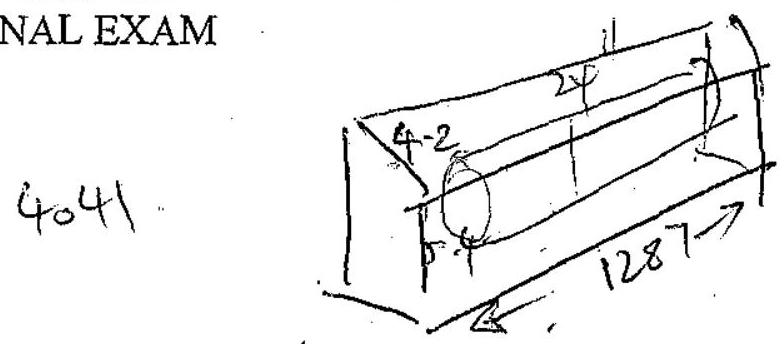
\includegraphics[max width=\textwidth]{2022_11_11_a5e8a54031fc138b833ag-1}

\begin{enumerate}
  \item The continuous exchange of water between the earth and the atmosphere is called the hydrologic cycle.\\

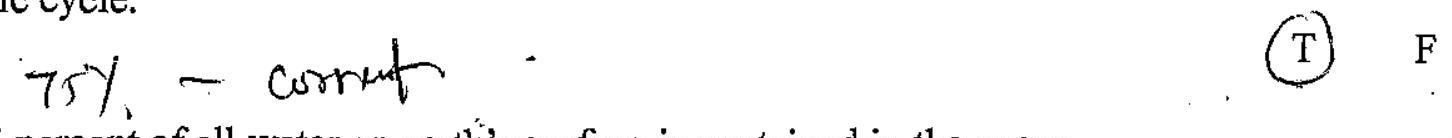
\includegraphics[max width=\textwidth]{2022_11_11_a5e8a54031fc138b833ag-1(1)}
\end{enumerate}

$=$ 2. About 85 percent of all water on earth's surface is contained in the ocean.

\begin{enumerate}
  \setcounter{enumi}{2}
  \item Hydraulics is a branch of the science that deals with liquids in motion or at rest.
\end{enumerate}

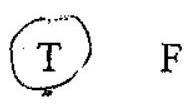
\includegraphics[max width=\textwidth]{2022_11_11_a5e8a54031fc138b833ag-1(2)}

\begin{enumerate}
  \setcounter{enumi}{3}
  \item The static suction head, plus friction suction head, plus the static discharge head, plus friction discharge head, make up the total dynamic head of a pump.

  \item Most of the pumps used in the water industry are of a positive displacement design.

\end{enumerate}

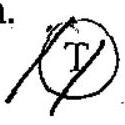
\includegraphics[max width=\textwidth]{2022_11_11_a5e8a54031fc138b833ag-1(3)}

\begin{enumerate}
  \setcounter{enumi}{5}
  \item A violation of primary drinking water standards may result in a health risk.

  \item Water maintenance personnel don't need to worry about customer relations, as long as the work gets done.

  \item Water meters of the multi-jet design are positive displacement meters.

\end{enumerate}


\includegraphics[max width=\textwidth]{2022_11_11_a5e8a54031fc138b833ag-1(4)}

\begin{enumerate}
  \setcounter{enumi}{8}
  \item A water distribution network should be designed with fire flow demands in mind.

  \item Wet barrel fire hydrants are always used in cold climates.

  \item The purpose of a jar test is to determine:\\
(A.) The correct amount of chemical to use for proper coagulation.\\
B. The amount of chlorine to add for breakpoint coagulation.\\
C. How long the water takes to fill the jar.\\
D. Length of time for the flash mix. 12. The branch of science which deals with water or fluids at rest or in motion is\\
A. conductivity\\
B. geology\\
C. oceanography\\
D. hydraulics

  \item Which is not a form of precipitation?\\
A. Snow\\
B. Rain\\
C. Hail\\
(D.) Water vapor

  \item The process by which water changes from vapor state to liquid state is called:\\
A. Evaporation\\
(B.) Condensation\\
c. Precipitation\\
D. Transpiration

  \item Pressure is usually measured in:\\
A. CFS\\
B. GPM\\
C. FT-LBS\\
(D.) PSI

  \item Disinfection is:\\
A. Killing all bacteria\\
B. Killing only protozoan\\
(C.) Killing pathogenic bacteria\\
D. All of the above

  \item The $\mathrm{pH}$ scale runs from:\\
A. $0-15$\\
(B.) $0-14$\\
D. $7-14$

  \item The major consideration in the design of a water storage and distribution system is\\
(A.) fire and maximum demand requirements\\
B. What the developer wants to pay\\
C. what type of pipe to use\\
D. none of the above

  \item A cross connection is:\\
A. A main line break\\
B. A connection between two safe water supplies\\
Where two mains intersect forming a cross\\
D. A connection between a potable water system and a source of unknown quality 20. A pH value of $7.0$ is considered to be:\\
A. Acidic\\
B. Alkaline\\
C. Base\\
(D.) Neutral

  \item A pH value of $8.0$ is considered to be:\\
A. Acidic\\
B. Alkaline\\
C. Potable\\
D. Neutral

  \item A pathogen is:\\
(A.) Disease causing\\
B. Cancer causing\\
C. Produces a smell like rotten eggs\\
D. A chemical used to fight algae

  \item A vertical turbine pump is typically used to pump water:\\
A. From a ditch\\
(B.) From a deep well\\
C. That contains rocks and trash\\
D. From one fire truck to another

  \item The difference between the static level and the pumping level of a well is called the:\\
A. Zone of saturation\\
B. Drawdown\\
C. Radius of influence\\
D. Cone of depression

  \item A well pumping into a reservoir at $1500 \mathrm{GPM}$ while water is being withdrawn from the reservoir at $1600 \mathrm{GPM}$. Which direction is the reservoir water level going?\\
A Up\\
B. Down\\
C. Stationary\\
D. None of the above

  \item The term "hot-tap" is used because\\
A. There is heat used in making the connection\\
(B.) the tap is done under pressure\\
C. such a tap is always welded on\\
D. none of the above 27. A water storage tank is 100 feet in diameter and is 40 feet in height. How many pounds of chlorine will be required to produce a dosage of 50 parts per million?\\
A. 980\\
B. 120\\
C. 1852\\
D. 440

  \item A rectangular reservoir is 140 feet long, 60 feet wide and 25 feet deep. If the inlet pipe flows at $545 \mathrm{GPM}$, how many days will the reservoir take to fill?\\
A. 2\\
B. $0.5$\\
C. 7\\
D. $2.8$

  \item One foot of water column creates a pressure of\\
A. $2.31 \mathrm{psi}$\\
B. $7.48 \mathrm{psi}$\\
(C) $0.433 \mathrm{psi}$\\
D. $0.785 \mathrm{psi}$

  \item "Aquifer" is the proper descriptive hydrologic term for:\\
A. Hydrophilic (water-loving) bacteria\\
B. All loose rock formations\\
C Vegetation along a stream bed\\
(D.) Water-bearing porous formations below the surface of the ground

  \item What type of respirator would be considered the best choice for use in the event of a chlorine gas leak repair?\\
(A.) $\mathrm{SCBA}$\\
B. Cartridge Respirator\\
C. Air Capsule

  \item Air/Vacuum relief valves work automatically and should be installed:\\
A. at the highest point in the water line\\
B. below ground for protection\\
(C.) on all the high points of a water line\\
D. at low areas for drainage

  \item A written Confined Space Program is required of all employers having more than seven employees and any workspace that:\\
A. has limited or restricted means of entry or exit\\
B. is large enough for an employee to enter and perform work\\
C is not designated for continuous work occupancy\\
(D.) any of the above 34. An Annual Consumer Confidence Report is required to be mailed to all customers under the Safe Drinking Water Act for all water systems the serve more than:\\
A. 100 mobile homes\\
B. 1,000 people\\
C.) 10,000 people\\
D. 5,000 people

  \item The overflow of a $30 \mathrm{MG}$ reservoir is at 1250 feet above sea level. If the reservoir is full and we place a gage on a hydrant at the $1050 \mathrm{ft}$. elevation', what will the pressure be in PSI, assuming no flow through the pipe?\\
(A.) $86.6$\\
C. 541\\
D. 114

\end{enumerate}

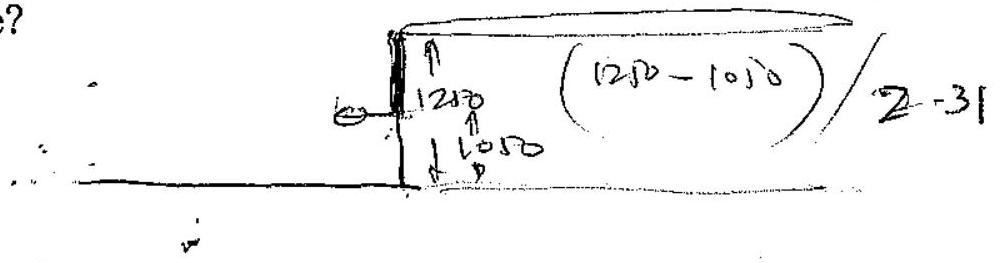
\includegraphics[max width=\textwidth]{2022_11_11_a5e8a54031fc138b833ag-5}

\begin{enumerate}
  \setcounter{enumi}{35}
  \item An 8 inch ductile iron pipeline is 1200 feet long. How many pounds of $70 \%$ calcium Hypochlorite would be required to disinfect at a dosage of 75 PPM?\\
(2) $1.96$\\
B. $4.0$\\
(C.) $2.80$\\
D. $5.26$\\

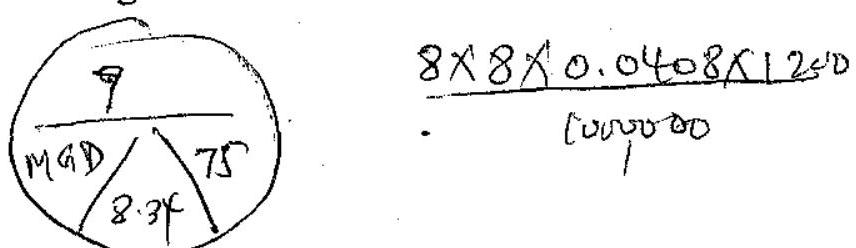
\includegraphics[max width=\textwidth]{2022_11_11_a5e8a54031fc138b833ag-5(1)}

  \item Determine the rate of flow in a 24 inch pipeline flowing full at a velocity of 6 feet per second. Give the answer on cubic feet per second.\\
A. $21.2$\\
B. $2.63$\\
(C.) $18.8$\\
D. $5.93$

\end{enumerate}

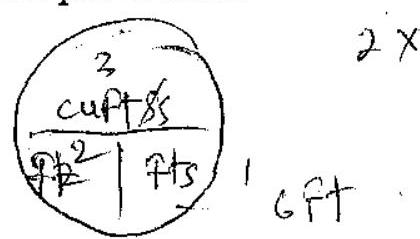
\includegraphics[max width=\textwidth]{2022_11_11_a5e8a54031fc138b833ag-5(2)}

$2 \times 2 \times 0.785 \times 6$


\includegraphics[max width=\textwidth]{2022_11_11_a5e8a54031fc138b833ag-5(3)}

\begin{enumerate}
  \setcounter{enumi}{37}
  \item A small water system produces 2 million gallons per day. What is the chlorine demand if the plant uses 11.7.lbs. of chlorine gas per day and the residual at the far end of the system is $0.5$ PPM?\\
A. $1.2$\\
B. $0.6$\\
(C.) $0.2$\\
D. $5.93$
\end{enumerate}

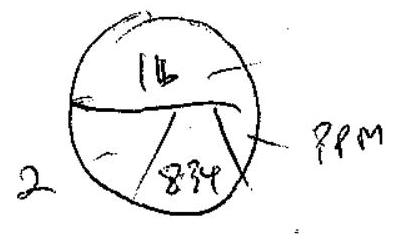
\includegraphics[max width=\textwidth]{2022_11_11_a5e8a54031fc138b833ag-5(4)}

\begin{enumerate}
  \setcounter{enumi}{38}
  \item If the pressure at a water main is $50 \mathrm{PSI}$, what would the static pressure be at a faucet on the top floor of a four story building? (Assuming $10 \mathrm{ft}$. per story)\\
A. $32.7$\\
B. $29.9$\\
C. $64.2$\\
D. $43.3$\\

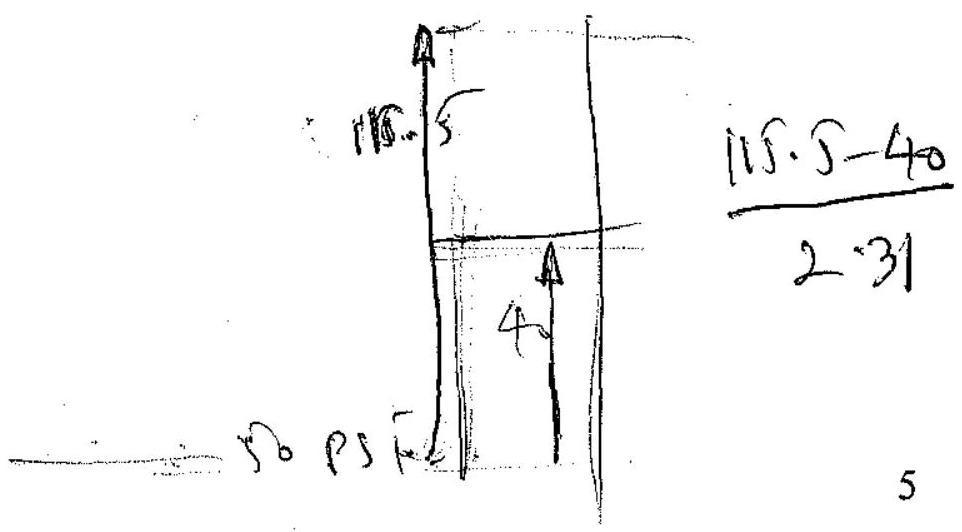
\includegraphics[max width=\textwidth]{2022_11_11_a5e8a54031fc138b833ag-5(5)}40. What is the amount of chlorine required to treat $5 \mathrm{MG}$ of water to provide a $0.8 \mathrm{PPM}$ residual And satisfy a 2.4 PPM chlorine demand?\\
A. $28.1$\\
B. $66.7$\\
C. 100\\
(D) 133\\

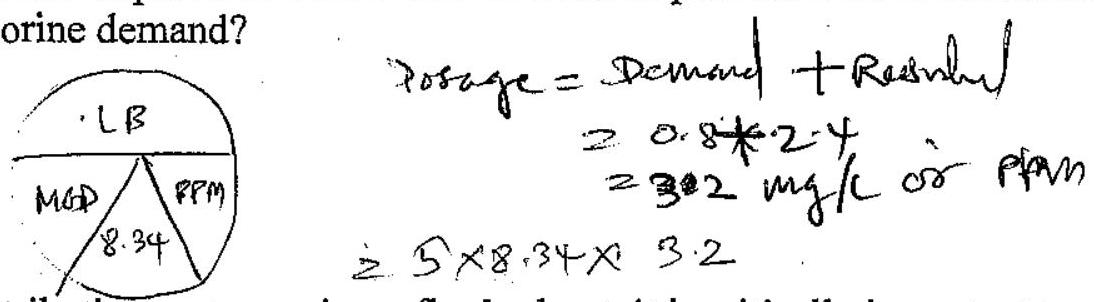
\includegraphics[max width=\textwidth]{2022_11_11_a5e8a54031fc138b833ag-6}

  \item When flushing a water distribution system using a fire hydrant, it is critically important to

\end{enumerate}

$$
=5 \times 834 \times 3.2
$$

A. Open valve fully\\
B. Close hydrant slowly to minimize hydraulic shock (water hammer)\\
C. Use the proper valve handle\\
D. Measure and record rate of flow, etc.

\begin{enumerate}
  \setcounter{enumi}{41}
  \item Modern SCADA systems would be best defined as :\\
A. Semi-automatic control\\
B. remote manual control\\
(ax) distributed computer control\\
D. centralized computer control

  \item In California, regardless of conditions, shoring is required in any trench where the depth is:\\
(A.) $5 \mathrm{feet}$\\
B. 4 feet\\
C. deeper than you can jump out of\\
D. 3 feet

\end{enumerate}

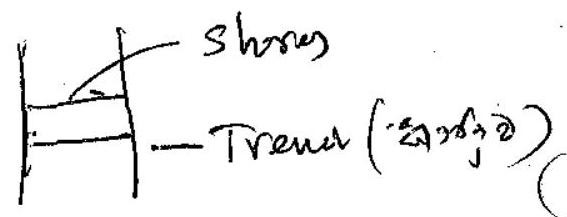
\includegraphics[max width=\textwidth]{2022_11_11_a5e8a54031fc138b833ag-6(1)}

\begin{enumerate}
  \setcounter{enumi}{43}
  \item The most serious potential problem that water distribution systems can experience during heaxy flows (such as during fire fighting) is:\\
(A.) Back-siphonage caused by negative pressures\\
B. Movement of buried pipes caused by surge\\
C. Loss of chlorine residual in system\\
D. Temporary dirty-water complaints
\end{enumerate}

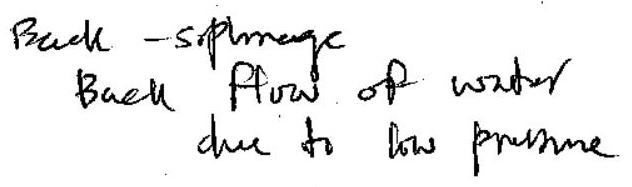
\includegraphics[max width=\textwidth]{2022_11_11_a5e8a54031fc138b833ag-6(2)}

\begin{enumerate}
  \setcounter{enumi}{44}
  \item When a positive coliform bacteria sample is found in a distribution system sample the utility must:\\
A. immediately notify the State Health Department office\\
B. resample the site within 24 hours\\
Cy sample upstream and downstream from the site within 24 hours\\
D.) all of the above

  \item A violation of primary DOHS standards is more critical than a violation of secondary standards due to the fact that:\\
(A.) primary standards are health related\\
B. secondary standards are health related

\end{enumerate}

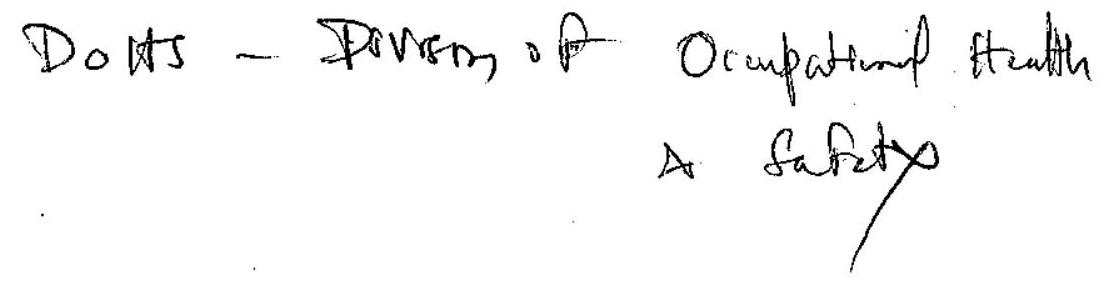
\includegraphics[max width=\textwidth]{2022_11_11_a5e8a54031fc138b833ag-6(3)}

\begin{enumerate}
  \setcounter{enumi}{46}
  \item A finished water reservoir is required to have:\\
A. a roof\\
B. locked entry hatches\\
(C.) screened vents\\
D. all of the above

  \item A new section of pipeline must be disinfected:\\
A. at the factory\\
B. after delivery to utility storage yards\\
(C.) after installation and prior to potable use\\
D. just before delivery to the site

  \item Centrifugal pumps are mainly used in the water industry because:\\
A. the are mechanically simple ".\\
B. the have a low starting torque\\
$\mathrm{C}$ they have a smooth operating range\\
(D.) all of the above

  \item Methemoglobinemia or blue- baby syndrome is oxygen starvation caused by:\\
A. too much chlorine\\
(B.) nitrates in the water\\
C. the house is too cold\\
D. none of the above

\end{enumerate}

\end{document}